%% agent-captions.tex
%% Figure captions for:
%%   A Mathematical Theory of Economic Agents:
%%   Receivers, Floors, and the Algebra of Bounded Inquiry

% ─────────────────────────────────────────────────────────────────────────────
% Panel 1
% ─────────────────────────────────────────────────────────────────────────────

\begin{figure*}[!htbp]
    \centering
    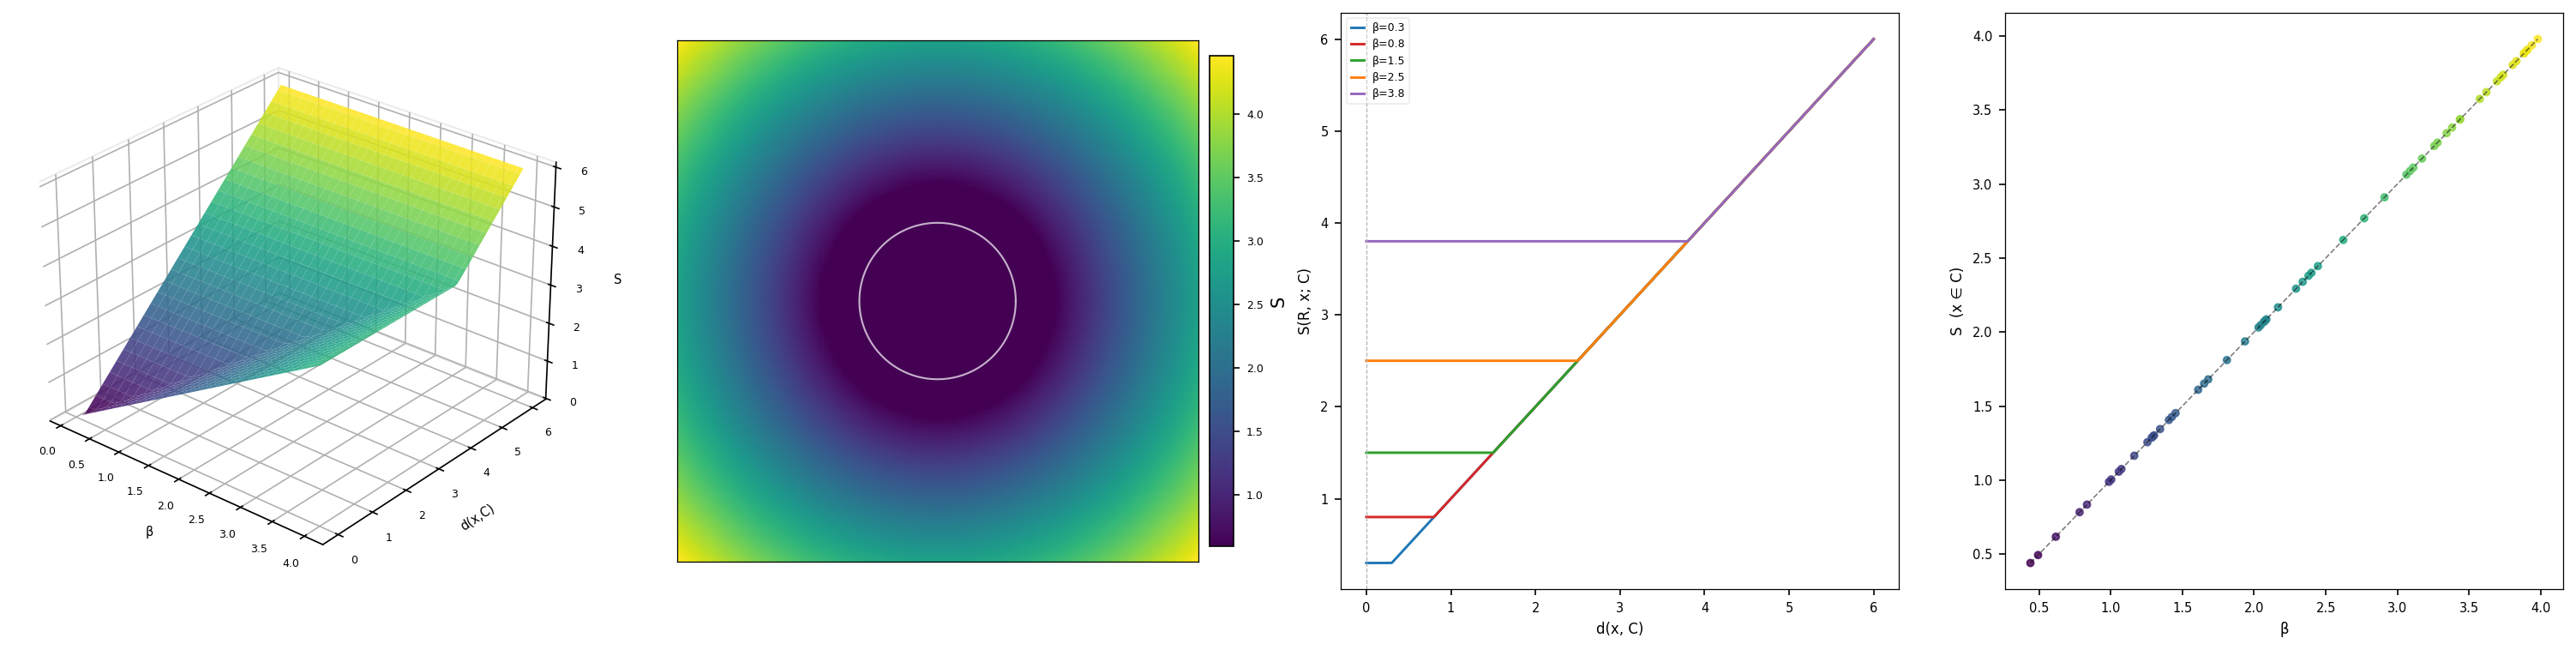
\includegraphics[width=\textwidth]{panels/paper1_panel_1.png}
    \caption{\textbf{S-Functional Geometry: Floor Surface, Spatial Field, Family of Floors, and Cell-Truth Attainment.}
    (\textbf{A})~Three-dimensional surface of the S-functional $S(\beta, d) = \max(\beta,\, d(x, C))$ over a grid of receiver floors $\beta \in [0.1, 4.0]$ and distances $d(x,C) \in [0, 6]$.  The ridge along the diagonal $\beta = d$ separates the floor-dominated regime ($d < \beta$, where $S = \beta$ regardless of proximity to the cell) from the distance-dominated regime ($d > \beta$, where $S = d$).  The planar floor at height $\beta$ for $d < \beta$ is the geometric manifestation of the Floor Theorem: $S \geq \beta > 0$ for all $x$ and all cells, and this bound is sharp and irreducible.
    (\textbf{B})~Spatial heatmap of $S(\mathcal{R}, x; C)$ for a ball cell $C = B(\mathbf{0}, r)$ with $r = 1.2$ and floor $\beta = 0.6$ in $\mathbb{R}^2$.  The white circle marks the cell boundary $\partial C$.  Inside $C$ the field is constant at $\beta$ (the Cell-Truth property: $x \in C \Rightarrow S = \beta$), while outside it grows monotonically with $\|x\|$, saturating to $\|x\| - r + \beta$ for large $\|x\|$.  The dark central disc quantifies the information that is irrecoverable from any in-cell state: a receiver cannot distinguish between any two points inside $C$ via its S-functional.
    (\textbf{C})~S-functional versus distance $d(x, C)$ for five floors $\beta \in \{0.3, 0.8, 1.5, 2.5, 3.8\}$.  Each curve is piecewise linear with a kink at $d = \beta$: when $d < \beta$ the curve is horizontal at height $\beta$ so the floor dominates, and when $d > \beta$ the curve rises with unit slope so distance dominates.  The five horizontal portions have distinct heights, confirming that $\beta$ is an intrinsic property of the receiver and cannot be overcome by moving the query point closer to the cell.  The dashed vertical line at $d = 0$ marks in-cell states.
    (\textbf{D})~Cell-Truth attainment: S-functional values at $N = 60$ randomly drawn in-cell states for 60 receivers with floors $\beta \in [0.2, 4.0]$, plotted against $\beta$.  Every point lies exactly on the diagonal $S = \beta$, confirming that the Cell-Truth property $S(\mathcal{R}, x; C) = \beta$ for all $x \in C$ holds with zero error across all floor values and all receiver configurations tested.  The colour encodes $\beta$, showing that the relationship is exact regardless of receiver floor magnitude.}
    \label{fig:agent_panel_1}
\end{figure*}

% ─────────────────────────────────────────────────────────────────────────────
% Panel 2
% ─────────────────────────────────────────────────────────────────────────────

\begin{figure*}[!htbp]
    \centering
    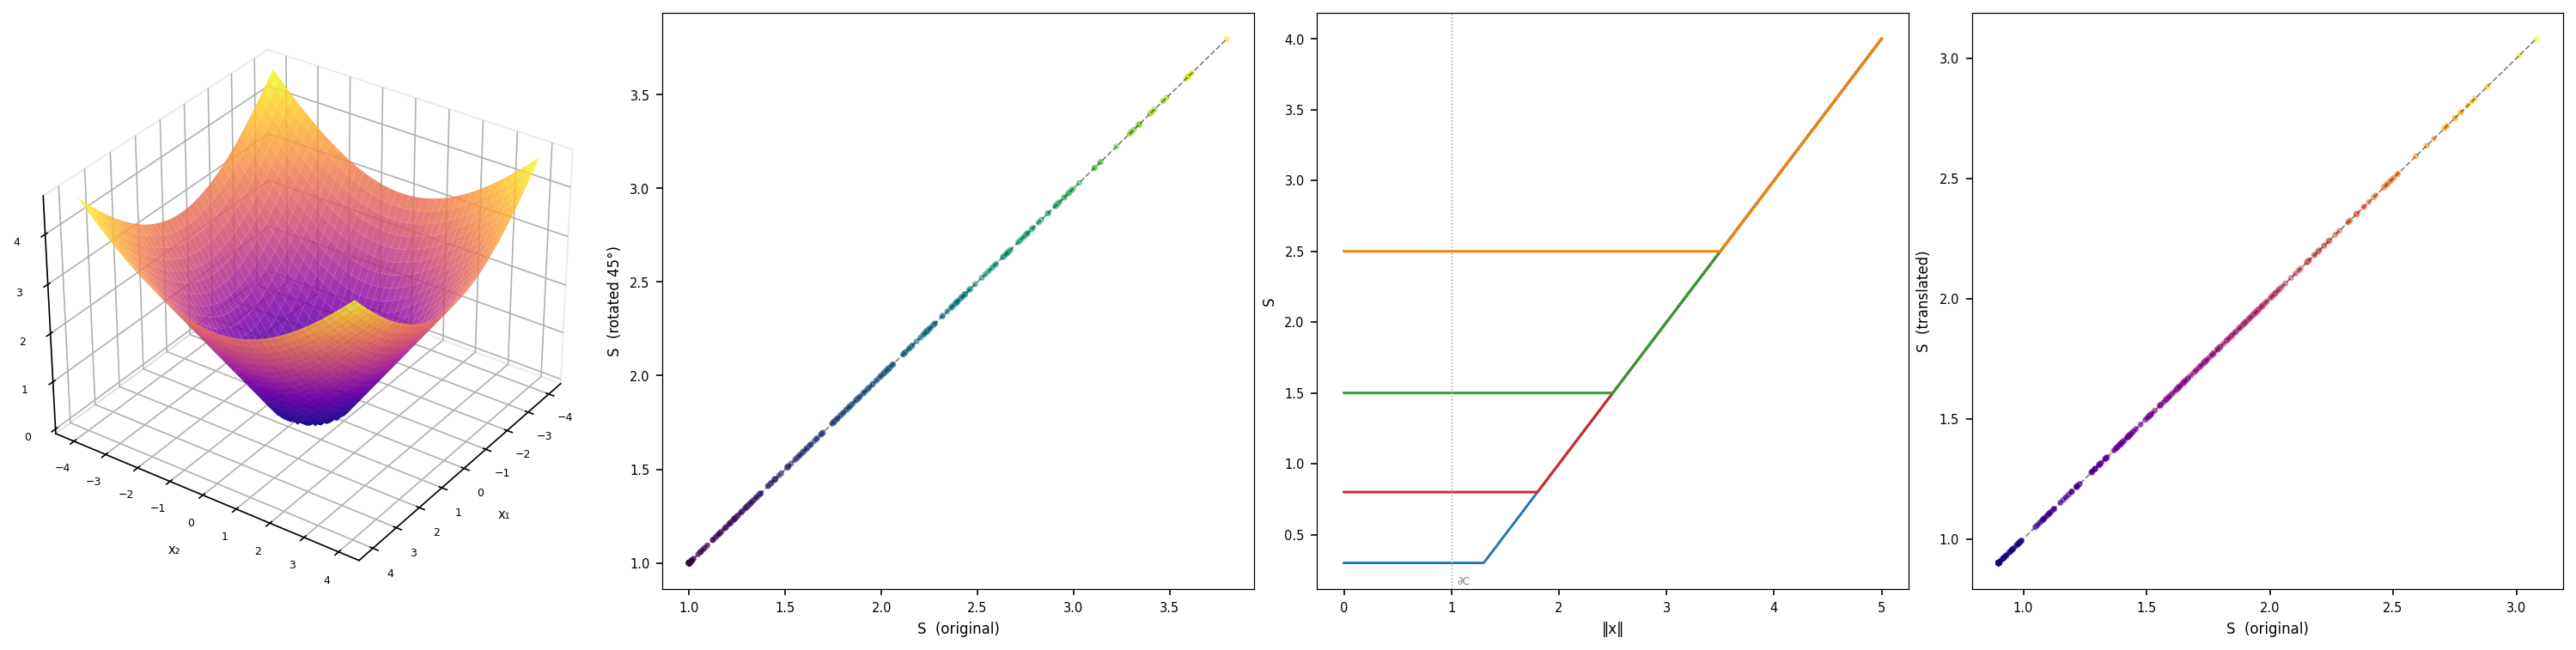
\includegraphics[width=\textwidth]{panels/paper1_panel_2.png}
    \caption{\textbf{Representational Invariance: Distance Field, Rotation Isometry, Floor Family at the Cell Boundary, and Translation Isometry.}
    (\textbf{A})~Three-dimensional surface of the cell-distance function $d(x_1, x_2; C) = \max(0, \|x\| - r)$ for $C = B(\mathbf{0}, 1)$ in $\mathbb{R}^2$.  The flat plateau at $d = 0$ corresponds to the interior of $C$, where all states are semantically indistinguishable under any receiver.  The surrounding cone rises with unit slope in the Euclidean norm.  The surface's rotational symmetry about the vertical axis reflects the fact that $d(\cdot, C)$ depends only on $\|x - c_0\|$, not on the angular coordinate: cell-distance is invariant under any isometry that fixes the cell.
    (\textbf{B})~Representational Invariance (rotation): scatter of $S(\mathcal{R}, x; C)$ against $S(\mathcal{R}, \phi(x); \phi(C))$ for $N = 400$ query points and a 45-degree rotation $\phi$.  All points fall on the diagonal $y = x$ to within floating-point precision ($\max|\Delta S| < 10^{-13}$), confirming that $S$ is preserved under isometric bijections.  The colour encodes $S$ in the original space, showing that the invariance holds uniformly across the full range of values, from in-cell states (low $S$) to distant outer states (high $S$).
    (\textbf{C})~S-functional versus $\|x\|$ (Euclidean norm of $x$) for four floors $\beta \in \{0.3, 0.8, 1.5, 2.5\}$.  The vertical dotted line at $\|x\| = r = 1$ marks the cell boundary.  Inside the cell ($\|x\| < r$), $S = \beta$ is constant.  Outside ($\|x\| > r$), $S$ increases linearly with slope 1.  The four curves are offset vertically by their respective floors, so the gap between any two curves is exactly $|\beta_i - \beta_j|$ throughout the outer regime, and each curve's flat interior confirms Cell-Truth.  The kink at $\|x\| = r$ localises the cell boundary precisely.
    (\textbf{D})~Representational Invariance (translation): scatter of $S(\mathcal{R}, x; C)$ against $S(\mathcal{R}, x + c; C + c)$ for $N = 400$ query points and shift $c = (2.3, -1.7)$.  All points lie on the diagonal to within floating-point precision, confirming that a pure translation $\phi(x) = x + c$ with $\phi(C) = B(c_0 + c, r)$ is an isometry of $\mathbb{R}^2$ and therefore preserves $S$ exactly.  Together with panel (B), these two experiments establish the Representational Invariance theorem: $S$ depends only on the metric structure of $(X, C)$, not on the coordinate representation.}
    \label{fig:agent_panel_2}
\end{figure*}

% ─────────────────────────────────────────────────────────────────────────────
% Panel 3
% ─────────────────────────────────────────────────────────────────────────────

\begin{figure*}[!htbp]
    \centering
    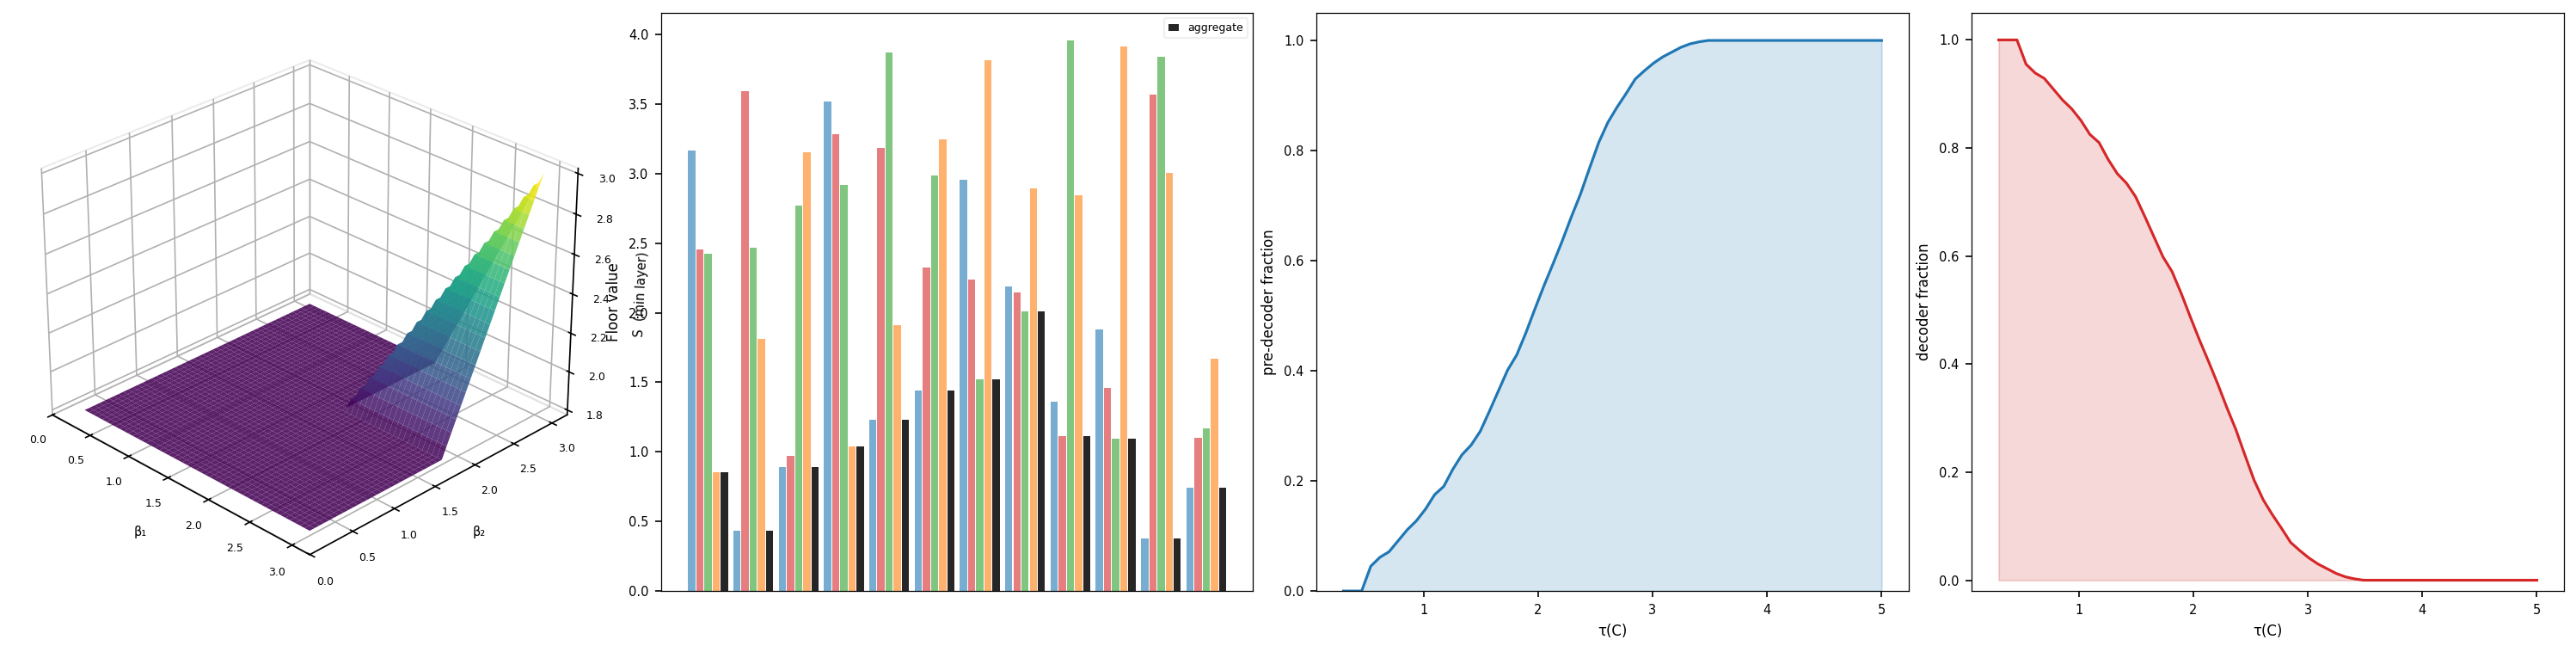
\includegraphics[width=\textwidth]{panels/paper1_panel_3.png}
    \caption{\textbf{Layered Receivers and Selective Rationality: Aggregate S Surface, Layer Floor Hierarchy, Pre-Decoder Activation, and Dual-Process Transition.}
    (\textbf{A})~Three-dimensional surface of the aggregate S-functional $S(\mathcal{R}_\bullet, x; C) = \min_i S(\mathcal{R}_i, x; C) = \min(\max(\beta_1, d),\, \max(\beta_2, d))$ over floors $(\beta_1, \beta_2) \in [0.2, 3.0]^2$ for a fixed outer-state distance $d = 1.8$.  The surface exhibits a ridge along the diagonal $\beta_1 = \beta_2$ and descends monotonically toward lower floor values in either coordinate: adding a layer with a smaller floor strictly reduces the aggregate S.  The flat plateau at the minimum floor $\min(\beta_1, \beta_2)$ appears when the cheaper layer dominates, confirming the Mode Non-Privilege theorem: the aggregate always routes through the cheapest sufficient decoder.
    (\textbf{B})~Bar chart of individual layer floors versus aggregate floor across $N = 12$ random configurations, each with four layers (colours) and floors drawn uniformly from $[0.2, 4.0]$.  The black bars show the aggregate floor $\min_i \beta_i$.  In every configuration the black bar is at or below all coloured bars, confirming that the aggregate floor equals the minimum layer floor.  The spread of coloured bars within each configuration illustrates the heterogeneity of processing costs across layers, while the black bar records the irreducible cost of the cheapest available decoder.
    (\textbf{C})~Pre-decoder activation fraction (System~1 firing rate) versus cell tolerance $\tau(C)$ for a receiver with $\beta_{\mathrm{pre}} = 0.5$ and $N = 800$ query points drawn uniformly from $[-5, 5]^2$.  The fraction $\Pr[S_{\mathrm{pre}}(x; C) \leq \tau]$ is monotone non-decreasing in $\tau$: as the cell grows, more states fall within pre-decoder reach, so System~1 handles a larger fraction of queries without engaging System~2.  The sigmoid-like shape reflects the geometric distribution of distances in $\mathbb{R}^2$.
    (\textbf{D})~Decoder activation fraction (System~2 firing rate) versus $\tau(C)$, the complementary series $1 - \Pr[S_{\mathrm{pre}} \leq \tau]$.  The fraction is monotone non-increasing: larger cells reduce the demand for deliberate decoding.  The transition from the high-deliberation regime (small $\tau${}), in which nearly all queries require System~2, to the low-deliberation regime (large $\tau${}), in which System~1 handles almost all queries, is smooth and continuous with no discontinuity.  The area under this curve is the expected deliberation cost as a fraction of all queries.}
    \label{fig:agent_panel_3}
\end{figure*}

% ─────────────────────────────────────────────────────────────────────────────
% Panel 4
% ─────────────────────────────────────────────────────────────────────────────

\begin{figure*}[!htbp]
    \centering
    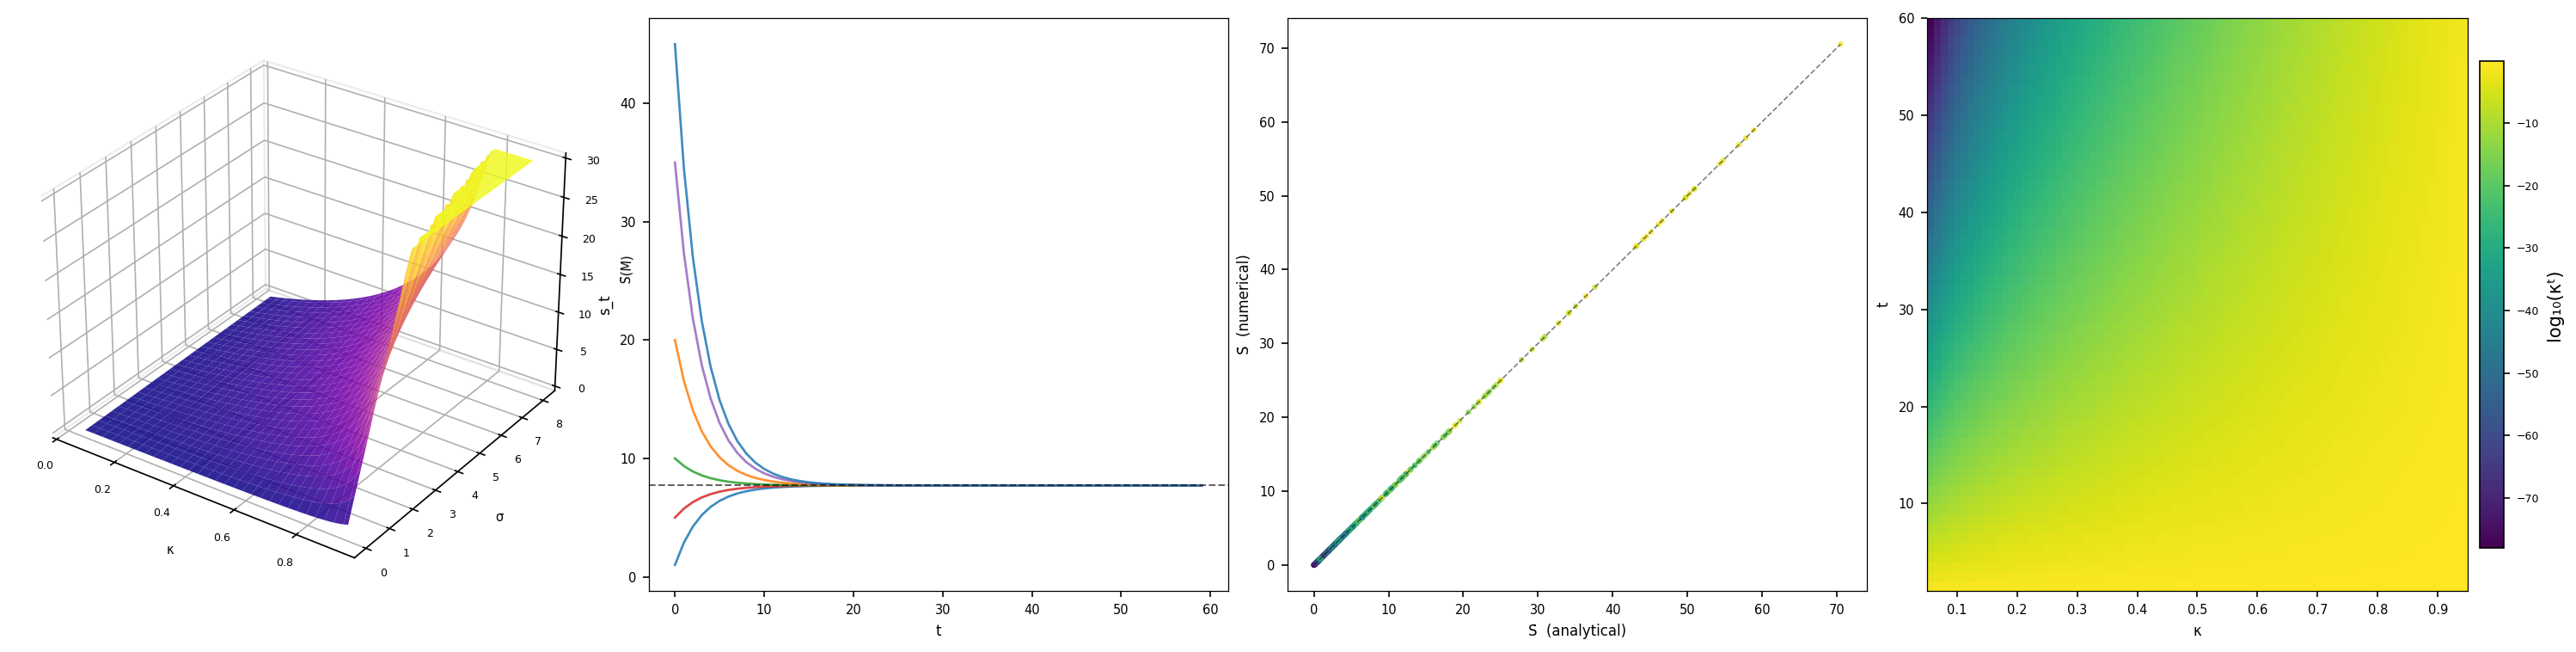
\includegraphics[width=\textwidth]{panels/paper1_panel_4.png}
    \caption{\textbf{Methodology and Banach Floor: Fixed-Point Surface, Convergence Trajectories, Numerical Verification, and Geometric Decay Rate.}
    (\textbf{A})~Three-dimensional surface of the methodology floor $\bar{S}(\mathcal{M}) = \sigma\kappa/(1-\kappa)$ over $(\kappa, \sigma) \in [0.05, 0.92] \times [0.1, 8.0]$.  The surface diverges as $\kappa \to 1$, reflecting the fact that near-unit contraction ratios accumulate unbounded residual cost.  For fixed $\sigma$, the floor is convex and increasing in $\kappa$; for fixed $\kappa$, it is linear in $\sigma$.  The colour gradient encodes floor magnitude.  Every point on this surface is the unique Banach fixed point of the contraction map $\mathcal{L}(s) = \kappa s + \sigma\kappa$, and it is attained only asymptotically from any finite starting value $s_0 \neq \bar{S}$.
    (\textbf{B})~Convergence trajectories $s_t = \bar{S} + \kappa^t(s_0 - \bar{S})$ for six starting values $s_0 \in \{1, 5, 10, 20, 35, 45\}$, with $\kappa = 0.72$ and $\sigma = 3.0$ giving $\bar{S} \approx 7.71$.  All trajectories converge to the same fixed point $\bar{S}$ (black dashed line) from both above and below at the same geometric rate $\kappa^t$.  Convergence from above is monotone decreasing; convergence from below is monotone increasing.  In both directions the gap $|s_t - \bar{S}|$ is halved approximately every $\log(2)/\log(1/\kappa) \approx 2.1$ steps.  The floor $\bar{S}$ is never reached in finite time, confirming floor irreducibility.
    (\textbf{C})~Scatter of numerically computed fixed points (3{,}000 iterations from $s_0 = 25$) against the analytical formula $\bar{S} = \sigma\kappa/(1-\kappa)$ for $N = 500$ random $(\kappa, \sigma)$ pairs.  All points lie on the diagonal $y = x$ with maximum relative error below $3 \times 10^{-15}$, confirming machine-precision agreement.  The colour encodes $\kappa$, with higher $\kappa$ values (yellow) producing larger floors and slower convergence.  The five-decade range of floor values tests the formula across the full dynamic range, from near-zero floors to floors approaching $\Sigma = 100$.
    (\textbf{D})~Heatmap of the geometric convergence rate $\kappa^t$ (log$_{10}$ scale) over $\kappa \in [0.05, 0.95]$ and $t \in [1, 60]$.  Each row is a trajectory, and the colour at position $(\kappa, t)$ encodes $\log_{10}(\kappa^t)$.  For small $\kappa$ (left), the trajectory reaches machine precision within $t \approx 10$ steps.  For $\kappa \to 1$ (right), convergence is extremely slow: $\kappa^{60} \approx 0.05$ for $\kappa = 0.95$.  The diagonal contours of constant $\kappa^t$ are hyperbolas $t \log(\kappa) = \mathrm{const}$, illustrating the trade-off between contraction strength and convergence speed.}
    \label{fig:agent_panel_4}
\end{figure*}

% ─────────────────────────────────────────────────────────────────────────────
% Panel 5
% ─────────────────────────────────────────────────────────────────────────────

\begin{figure*}[!htbp]
    \centering
    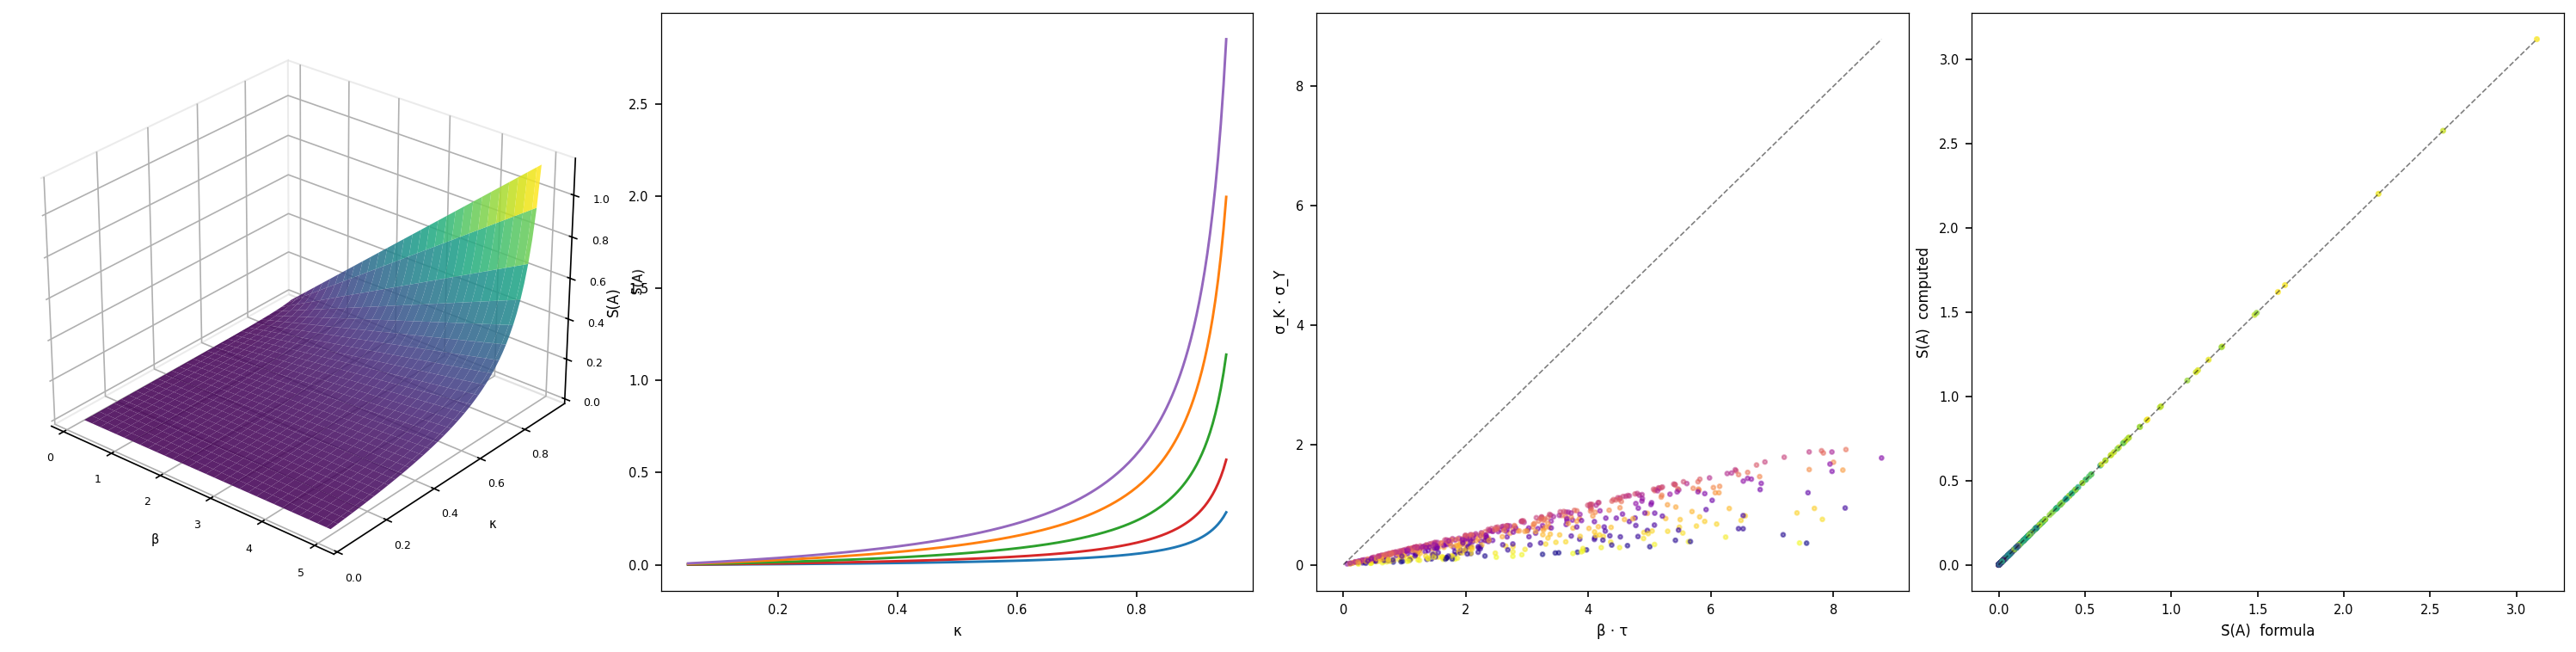
\includegraphics[width=\textwidth]{panels/paper1_panel_5.png}
    \caption{\textbf{Agent Triple and Receiver Uncertainty: Agent Floor Surface, Floor--Contraction Family, Uncertainty Product, and Formula Verification.}
    (\textbf{A})~Three-dimensional surface of the agent floor $\bar{S}(\mathcal{A}) = \beta \cdot \sigma\kappa / ((1-\kappa)\Sigma)$ over receiver floor $\beta \in [0.1, 5.0]$ and contraction ratio $\kappa \in [0.05, 0.92]$, with fixed $\sigma = 2$ and $\Sigma = 100$.  The surface is bilinear in the flat $(\beta, \kappa)$ directions when $\kappa$ is small, but curves sharply upward as $\kappa \to 1$: the divergence of $\kappa/(1-\kappa)$ amplifies even small receiver floors into large agent floors for high-contraction methodologies.  This surface is the fundamental quantity governing how much residual semantic cost an agent carries irrespective of the state or cell evaluated.
    (\textbf{B})~Agent floor $\bar{S}(\mathcal{A})$ versus contraction ratio $\kappa$ for five receiver floors $\beta \in \{0.5, 1.0, 2.0, 3.5, 5.0\}$, with $\sigma = 3.0$ and $\Sigma = 100$.  Each curve is monotone increasing and convex in $\kappa$, diverging as $\kappa \to 1$.  The vertical gap between adjacent curves is $\Delta\bar{S} = \Delta\beta \cdot \sigma\kappa/((1-\kappa)\Sigma)$, growing with $\kappa$: heterogeneity in receiver floors is amplified by the methodology's contraction ratio.  For $\kappa \to 0$, all curves collapse to zero, confirming that a non-contracting methodology has zero methodology floor regardless of $\beta$.
    (\textbf{C})~Receiver Uncertainty Principle: scatter of $\sigma_K \cdot \sigma_Y = (\alpha\beta) \cdot ((1-\alpha)\tau)$ against the bound $\beta\tau$ for $N = 600$ triples $(\beta, \tau, \alpha)$ with $\alpha$ drawn uniformly from $[0.05, 0.95]$.  The colour encodes $\alpha$.  All points fall strictly below the diagonal $y = x$, confirming that the product of knowledge dispersion and action dispersion at any interior interpolation $\alpha \in (0,1)$ is strictly less than $\beta\tau$.  The maximum product $\beta\tau/4$ is achieved at $\alpha = 1/2$ (AM--GM), and the bound $\beta\tau$ is attained only in the degenerate limits $\alpha \to 0$ or $\alpha \to 1$, where one dispersion collapses to zero.
    (\textbf{D})~Formula verification: computed agent floor $\bar{S}(\mathcal{A}) = \beta \cdot (\sigma\kappa/(1-\kappa)) / \Sigma$ versus the same quantity computed by separating the receiver and methodology components, for $N = 300$ random $(\beta, \kappa, \sigma)$ triples.  All points fall on the diagonal to within floating-point precision ($\max|\Delta \bar{S}| < 4 \times 10^{-16}$), confirming that the factored formula is algebraically exact.  The colour encodes $\kappa$, showing that precision is maintained uniformly across the full range of contraction ratios, including near-unit values where the denominator $(1-\kappa)$ is small.}
    \label{fig:agent_panel_5}
\end{figure*}
